\documentclass[10pt,a4paper]{paper}
\usepackage[utf8]{inputenc}
\usepackage[english]{babel}
\usepackage{tikz}
\usepackage{amsmath}
\usepackage{amsfonts}
\usepackage{amssymb}
\usepackage{bm}
\usepackage{geometry}
\usepackage{booktabs}
\usepackage{array}
\usepackage{graphicx}
\usepackage{subcaption}

\geometry{margin=1in}

% Paragraphs
\setlength{\parindent}{4pt}

% Title block: the paper class sets it flush left and does not print the date
\makeatletter
\def\@maketitle{%
  \null
  \vskip \beforetitlespace
  \begin{center}
    {\t@font \@title \par}%
    \vskip 1.5em
    {\a@font \lineskip .5em \begin{tabular}[t]{c}\@author\end{tabular}\par}%
    \vskip 1em
    {\large \@date \par}%
  \end{center}
  \par \vskip 1.5em
}
\makeatother

% Notation
\newcommand{\vb}{v}                                  % bare Coulomb interaction
\newcommand{\vemb}{v_{\mathrm{emb}}}                 % embedding term (reaction field of the literature)
\newcommand{\vt}{\tilde{v}}                          % dressed interaction v + v_emb
\newcommand{\chiL}{\chi^{\mathrm{L}}}                % response of the layer
\newcommand{\chiS}{\chi^{\mathrm{S}}}                % response of the substrate
\newcommand{\chiLt}{\tilde{\chi}^{\mathrm{L}}}       % layer response with the dressed interaction
\newcommand{\Qp}{Q}                                  % |q + G_par|
\newcommand{\gs}{g}                                  % surface response function of the substrate
\newcommand{\epsenv}{\varepsilon_{\mathrm{env}}}     % effective dielectric function of the environment
\newcommand{\rpar}{\bm{r}_{\parallel}}               % in-plane position
\newcommand{\Qv}{\bm{Q}}                             % in-plane wave vector


\title{Effective substrate screening in GW and BSE calculations of 2D layers}
\author{Marco D'Alessandro}
\date{\today}

\begin{document}
\maketitle

\section{Introduction}
\label{sec:intro}

These notes describe how the dielectric screening of a bulk substrate can be included, in an effective way, in GW
and Bethe--Salpeter (BSE) calculations of a two-dimensional layer physisorbed on it. The layer is computed alone in
a periodic supercell, and the substrate never appears explicitly in the calculation. We consider the simplest
situation, in which layer and substrate interact only through their mutual polarization: there is no charge
transfer and no hybridization between their states. The first system we have in mind is germanene on hexagonal
boron nitride.

When the wavefunctions of the two subsystems do not overlap, the independent-particle response is the sum of the
responses of the layer and of the substrate, $\chi_0 = \chi_0^{\mathrm{L}} + \chi_0^{\mathrm{S}}$. The substrate
then enters the many-body problem of the layer only through a reaction field that dresses the bare Coulomb
interaction~\cite{amblard2023many,amblard2024static,duchemin2024polarizable},
\begin{equation}
\vt = \vb + \vreac , \qquad \vreac = \vb\,\chiS\,\vb ,
\label{eq:vtilde}
\end{equation}
where $\chiS$ is the interacting response of the substrate alone. The aim of this work is to build $\vreac$ for a
semi-infinite substrate and to use it in the GW and BSE calculations of the layer, acting on the databases of the
many-body code rather than on its source.

\section{A sheet of oscillators above a dielectric substrate}
\label{sec:modelA}

Before turning to the many-body problem we study the simplest classical model that contains the physics of
Eq.~\eqref{eq:vtilde}: a thin sheet of identical charged harmonic oscillators placed at a distance $d$ above a
semi-infinite substrate with a static and local dielectric constant $\varepsilon$. The substrate stands for the
electronic polarization of a wide-gap insulator, whose excitations lie well above the frequencies of the sheet. We
work in the quasi-static limit (retardation neglected, valid for in-plane wave vectors $Q \gg \omega/c$). The
question is how the substrate modifies the interaction between the oscillators and their resonances. We first
discuss how a charge distribution in a plane and its Coulomb potential are described in terms of in-plane wave
vectors, which is the language used in the rest of these notes.

The electrostatics is written in SI form, $\nabla^2\phi = -\rho/\varepsilon_0$. The Hartree atomic units of the
many-body part follow from $e = m = \hbar = 4\pi\varepsilon_0 = 1$, that is from the replacement
$1/\varepsilon_0 \to 4\pi$.

\subsection{Charges in a plane: charge waves and their potential}
\label{sec:charge_wave}

\paragraph{Charge waves.} Consider a charge distribution confined to the plane $z = 0$, with zero thickness and
surface density $\sigma(\rpar)$ (charge per unit area): $\rho(\bm{r}) = \sigma(\rpar)\,\delta(z)$, with
$\bm{r} = (\rpar, z)$. We take the plane as a large square of area $A$ with periodic boundary conditions, so that the
in-plane wave vectors $\Qv$ form a discrete set with spacing $2\pi/\sqrt{A}$, and expand the surface density in
plane waves:
\begin{equation}
\rho(\bm{r}) = \frac{1}{A}\sum_{\Qv}\sigma_{\Qv}\,e^{i\Qv\cdot\rpar}\,\delta(z) , \qquad
\sigma_{\Qv} = \int_A d^2r_{\parallel}\;\sigma(\rpar)\,e^{-i\Qv\cdot\rpar} .
\label{eq:rho_waves}
\end{equation}
Each term of the sum is a \emph{charge wave} with wave vector $\Qv$, wavelength $\lambda = 2\pi/Q$ and $Q = |\Qv|$.
\begin{itemize}
\item The charge is real, so $\sigma_{-\Qv} = \sigma_{\Qv}^*$, and the waves $\pm\Qv$ add up to
  $(2|\sigma_{\Qv}|/A)\cos(\Qv\cdot\rpar + \theta_{\Qv})$, with $\theta_{\Qv}$ the phase of $\sigma_{\Qv}$: stripes
  normal to $\Qv$, alternately positive and negative, each of width $\lambda/2$.
\item Since $\int_A d^2r_{\parallel}\,e^{i\Qv\cdot\rpar} = A\,\delta_{\Qv,\bm{0}}$, a wave with $\Qv \neq 0$ contains
  as much positive as negative charge. The net charge of the plane is carried by the term $\Qv = 0$ alone:
  $\sigma_{\bm{0}} = \int_A d^2r_{\parallel}\,\sigma$ is the total charge and $\bar{\sigma} = \sigma_{\bm{0}}/A$ the
  average surface density. The waves with $\Qv \neq 0$ describe how the charge is distributed in the plane around
  this average.
\item A point charge $q$ at the origin, $\sigma = q\,\delta(\rpar)$, has $\sigma_{\Qv} = q$ for every $\Qv$. The
  term $\Qv = 0$ spreads the charge uniformly over the area $A$; the other waves, which add up in phase at the origin
  and cancel elsewhere, gather it into a point.
\item In a crystalline layer the wave vectors are written $\Qv = \bm{q} + \bm{G}_{\parallel}$, with $\bm{q}$ in the
  two-dimensional Brillouin zone and $\bm{G}_{\parallel}$ a reciprocal lattice vector, as in plane-wave codes. A
  density with the periodicity of the lattice, such as the ground-state density of the layer, has only the
  components $\bm{q} = 0$, $\Qv = \bm{G}_{\parallel}$: the term $\bm{G}_{\parallel} = 0$ is its average and those
  with $\bm{G}_{\parallel} \neq 0$ its modulation within the unit cell. Components with $\bm{q} \neq 0$ describe
  perturbations without the periodicity of the lattice, such as an added charge or an induced density wave.
\end{itemize}
For a large area the sum becomes an integral, $A^{-1}\sum_{\Qv} \to \int d^2Q/(2\pi)^2$.

\paragraph{Poisson equation for each wave.} The potential is expanded in the same way,
\begin{equation}
\phi(\bm{r}) = \frac{1}{A}\sum_{\Qv}\phi_{\Qv}(z)\,e^{i\Qv\cdot\rpar} .
\end{equation}
The two factors of each term depend on separate coordinates, so $\partial_z^2$ acts only on $\phi_{\Qv}(z)$ and the
in-plane derivatives only on the exponential (there are no mixed terms):
$\nabla^2[\phi_{\Qv}(z)\,e^{i\Qv\cdot\rpar}] = [\phi''_{\Qv}(z) - Q^2\phi_{\Qv}(z)]\,e^{i\Qv\cdot\rpar}$. Since plane
waves with different $\Qv$ are linearly independent, the Poisson equation $\nabla^2\phi = -\rho/\varepsilon_0$ splits
into one ordinary differential equation for each wave vector:
\begin{equation}
\phi''_{\Qv}(z) - Q^2\,\phi_{\Qv}(z) = -\frac{\sigma_{\Qv}}{\varepsilon_0}\,\delta(z) .
\label{eq:poisson_Q}
\end{equation}
The potential at wave vector $\Qv$ is produced only by the charge at the same wave vector: the waves are independent.
This is a consequence of the translational invariance of empty space along the plane, and it holds also in the
presence of a substrate that is homogeneous in the plane.

\paragraph{Conditions at the plane.} Away from the plane the right-hand side of Eq.~\eqref{eq:poisson_Q} vanishes.
The plane is crossed by integrating Eq.~\eqref{eq:poisson_Q} over a thin slab $-\eta < z < \eta$:
\begin{equation}
\phi'_{\Qv}(\eta) - \phi'_{\Qv}(-\eta) - Q^2\int_{-\eta}^{\eta}\phi_{\Qv}(z)\,dz
= -\frac{\sigma_{\Qv}}{\varepsilon_0} .
\end{equation}
For $\eta \to 0$ the integral of the finite potential vanishes: the $\delta$ function of the charge must be balanced
by a step of $\phi'_{\Qv}$, while $\phi_{\Qv}$ itself is continuous (a step of $\phi_{\Qv}$ would give a $\delta$ in
$\phi'_{\Qv}$ and a $\delta'$ in $\phi''_{\Qv}$, the charge of a double layer of dipoles, which is not present). The
two matching conditions are therefore
\begin{equation}
\phi_{\Qv}(0^+) = \phi_{\Qv}(0^-) , \qquad
\phi'_{\Qv}(0^+) - \phi'_{\Qv}(0^-) = -\frac{\sigma_{\Qv}}{\varepsilon_0} .
\label{eq:jump}
\end{equation}
Their meaning is clearer in terms of the field $\bm{E} = -\nabla\phi$, whose component at wave vector $\Qv$ is
$\bm{E}_{\Qv}(z) = -i\Qv\,\phi_{\Qv}(z) - \hat{\bm{z}}\,\phi'_{\Qv}(z)$. The first condition says that the
tangential field is continuous across the plane. The second says that the normal field jumps by the surface charge,
$E_{z,\Qv}(0^+) - E_{z,\Qv}(0^-) = \sigma_{\Qv}/\varepsilon_0$, or, summing over $\Qv$,
$E_z(\rpar,0^+) - E_z(\rpar,0^-) = \sigma(\rpar)/\varepsilon_0$ at every point of the plane. This is Gauss's law for
a flat box enclosing a small piece of the plane: the flux of $\bm{E}$ through its upper and lower faces is the
enclosed charge divided by $\varepsilon_0$, and the lateral faces do not contribute when the box is thin. Field lines
start on the positive charges of the plane and end on the negative ones; the jump of $\phi'$ measures how many lines
start or end at each point.

\paragraph{The uniform component, $\Qv = 0$.} For $\Qv = 0$ Eq.~\eqref{eq:poisson_Q} reads
$\phi''_{\bm{0}} = -(\sigma_{\bm{0}}/\varepsilon_0)\,\delta(z)$, so the potential is linear in $z$ on each side of
the plane. The conditions~\eqref{eq:jump} give $\phi_{\bm{0}}(z) = c - \sigma_{\bm{0}}|z|/(2\varepsilon_0)$, with
$c$ an arbitrary constant, and the contribution of this component to the potential and to the field is
\begin{equation}
\frac{\phi_{\bm{0}}(z)}{A} = \frac{c}{A} - \frac{\bar{\sigma}}{2\varepsilon_0}\,|z| , \qquad
\bm{E} = \frac{\bar{\sigma}}{2\varepsilon_0}\,\mathrm{sgn}(z)\,\hat{\bm{z}} ,
\label{eq:phi_uniform}
\end{equation}
the field of a uniformly charged infinite plane (Fig.~\ref{fig:charge_wave_field}a): uniform on each side, normal to
the plane and pointing away from it for $\bar{\sigma} > 0$, with half of the flux going up and half going down. It
never decays, the potential grows linearly with the distance, and the constant $c$ cannot be fixed by requiring the
potential to vanish far away: an infinite charged plane has no finite potential with respect to infinity.

In a neutral layer the charge of the electrons compensates that of the nuclei and $\sigma_{\bm{0}} = 0$: the uniform
component is absent. This is a consequence of neutrality, not of periodicity (the waves with $\Qv \neq 0$ carry no
net charge). Each species alone would form a uniformly charged plane with the field of Eq.~\eqref{eq:phi_uniform};
in periodic calculations these $\bm{G} = 0$ contributions cancel and are dropped, and the average potential, like
$c$ here, remains arbitrary.

\paragraph{A charge wave, $\Qv \neq 0$.} Away from the plane the solutions are $e^{\pm Qz}$. With no other charges
the potential must vanish far from the plane, which selects $e^{-Qz}$ above and $e^{Qz}$ below; continuity at
$z = 0$ requires the same amplitude $C$ on the two sides, so $\phi_{\Qv}(z) = C\,e^{-Q|z|}$. Its derivative jumps
from $+QC$ at $0^-$ to $-QC$ at $0^+$, and the second condition~\eqref{eq:jump}, $-2QC = -\sigma_{\Qv}/\varepsilon_0$,
fixes the amplitude:
\begin{equation}
\phi_{\Qv}(z) = \frac{\sigma_{\Qv}}{2\varepsilon_0 Q}\,e^{-Q|z|} .
\label{eq:phi_free}
\end{equation}
At the plane the normal field is $E_{z,\Qv}(0^\pm) = \pm\sigma_{\Qv}/(2\varepsilon_0)$: as for the uniform plane,
half of the field lines go up and half go down. The difference is that the lines leaving a positive stripe end on
the neighbouring negative stripes, so the field decays as $e^{-Q|z|}$ instead of extending to infinity
(Fig.~\ref{fig:charge_wave_field}b). For small $Q$,
\begin{equation}
\phi_{\Qv}(z) = \frac{\sigma_{\Qv}}{2\varepsilon_0 Q} - \frac{\sigma_{\Qv}}{2\varepsilon_0}\,|z| + O(Q) :
\label{eq:phi_smallQ}
\end{equation}
close to the plane ($|z| \ll 1/Q$) a long-wavelength wave looks like a uniformly charged plane, and its potential is
that of Eq.~\eqref{eq:phi_uniform} plus a constant. The constant, left arbitrary at $\Qv = 0$, is fixed here by the
decay of the field at $|z| \gtrsim 1/Q$, and it diverges as $1/Q$ because that distance does.

\begin{figure}[h!]
\centering
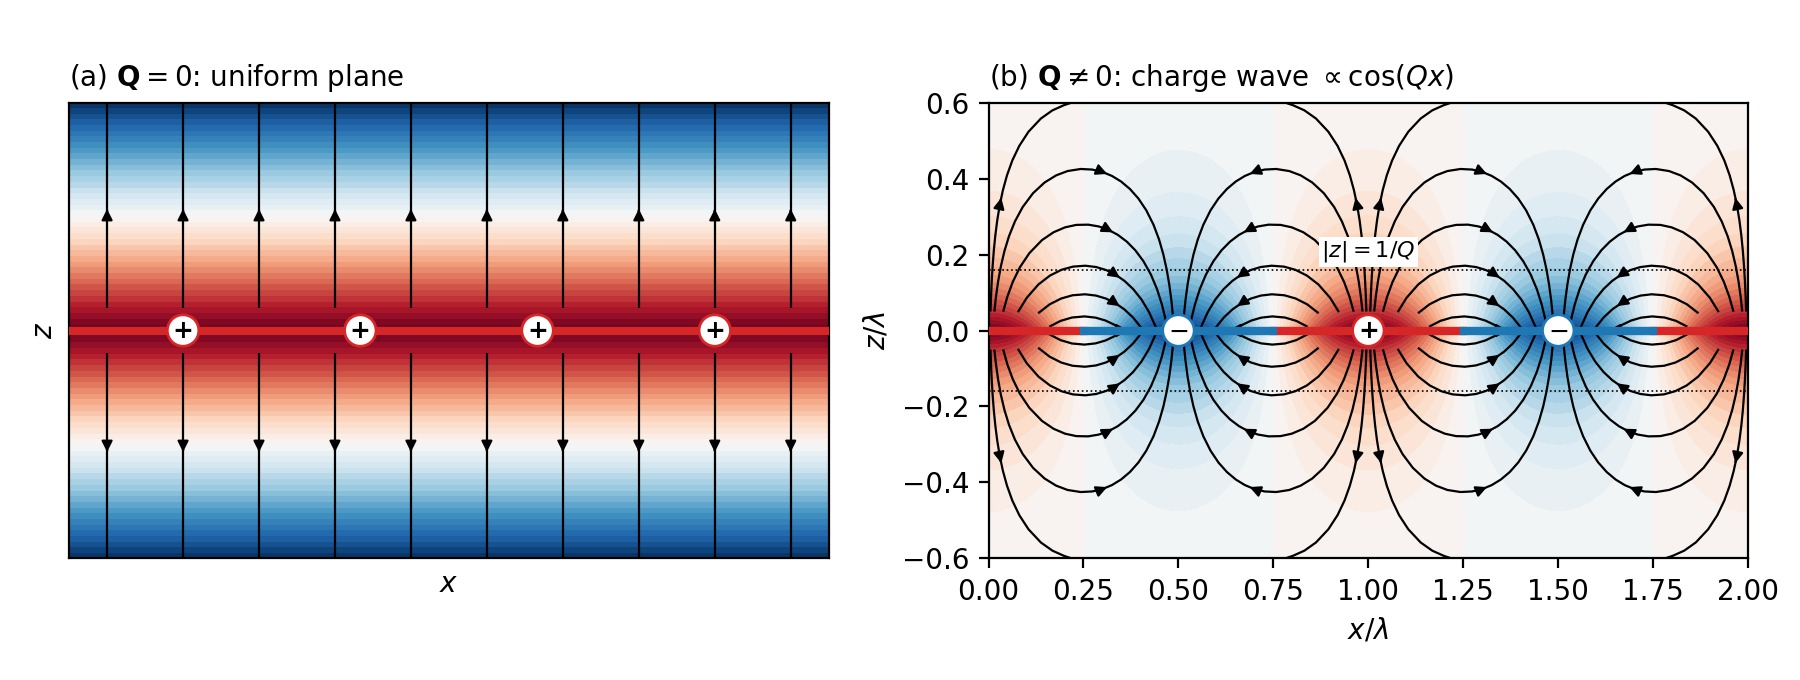
\includegraphics[width=\textwidth]{Figures/charge_wave_field.jpeg}
\caption{Field lines (black) and potential (colour: red positive, blue negative, arbitrary units) of a charged
plane at $z = 0$. (a) Uniform density, $\Qv = 0$, Eq.~\eqref{eq:phi_uniform}: the field is uniform on each side and
the potential decreases linearly with $|z|$ (its constant is arbitrary). (b) Charge wave $\propto \cos(Qx)$, sum of
the waves $\pm\Qv$ of Eq.~\eqref{eq:phi_free}: the field lines go from the positive to the negative stripes, and the
potential decays as $e^{-Q|z|}$; the dotted lines mark $|z| = 1/Q = \lambda/2\pi$.}
\label{fig:charge_wave_field}
\end{figure}

\paragraph{Coulomb interaction in the plane.} Summing the waves, the potential of any charge distribution in the
plane is
\begin{equation}
\phi(\bm{r}) = \frac{1}{A}\sum_{\Qv \neq 0}\frac{\sigma_{\Qv}}{2\varepsilon_0 Q}\,e^{-Q|z|}\,e^{i\Qv\cdot\rpar}
+ \frac{\phi_{\bm{0}}(z)}{A} .
\label{eq:phi_total}
\end{equation}
In the plane each wave produces a potential proportional to its own charge,
\begin{equation}
\phi_{\Qv}(0) = v(Q)\,\sigma_{\Qv} , \qquad v(Q) = \frac{1}{2\varepsilon_0 Q}
\quad \left(= \frac{2\pi}{Q} \text{ in atomic units}\right) .
\label{eq:v2d}
\end{equation}
For the point charge, $\sigma_{\Qv} = q$, and for a large area Eq.~\eqref{eq:phi_total} gives back the Coulomb
potential in the whole space,
\begin{equation}
q\int\frac{d^2Q}{(2\pi)^2}\,\frac{e^{-Q|z|}}{2\varepsilon_0 Q}\,e^{i\Qv\cdot\rpar}
= \frac{q}{4\pi\varepsilon_0\sqrt{|\rpar|^2 + z^2}}
\label{eq:v2d_ft}
\end{equation}
(the angular integral gives the Bessel function $J_0(Q|\rpar|)$, and
$\int_0^\infty dQ\,J_0(Qr)\,e^{-Q|z|} = (r^2 + z^2)^{-1/2}$). The term $\Qv = 0$, of order $q/A$, vanishes in this
limit: the long-range tail of the potential at a distance $|\rpar|$ is carried by the waves with
$Q \lesssim 1/|\rpar|$. Hence $v(Q)$ is the in-plane Fourier transform of the Coulomb kernel
$v(r) = 1/(4\pi\varepsilon_0 r)$, the potential of a unit charge (two charges $q_1$ and $q_2$ interact with energy
$q_1q_2\,v$; in atomic units, with $e = 1$, $v$ is the electron--electron interaction of the many-body problem). It
is not a different, two-dimensional law: it is the three-dimensional Coulomb interaction written in the mixed
representation $(\Qv, z)$, for two charges in the same plane. It follows from the bulk form
$1/(\varepsilon_0 k^2)$, with $\bm{k} = (\Qv, k_z)$, by integration over the out-of-plane wave vector,
$\int dk_z\,(2\pi)^{-1}\,e^{ik_zz}/[\varepsilon_0(Q^2 + k_z^2)] = e^{-Q|z|}/(2\varepsilon_0 Q)$.

The main features of the Coulomb interaction at finite $Q$ are the following.
\begin{itemize}
\item \emph{Range out of the plane.} For $\Qv$ along $x$ the field of a wave has components
  $E_x = -iQ\,\phi_{\Qv}(z)\,e^{i\Qv\cdot\rpar}$ and
  $E_z = (\sigma_{\Qv}/2\varepsilon_0)\,\mathrm{sgn}(z)\,e^{-Q|z|}e^{i\Qv\cdot\rpar}$. The field lines leave the
  positive stripes and end on the neighbouring negative ones, running through the half-spaces above and below the
  plane (Fig.~\ref{fig:charge_wave_field}b). They close within a distance of order $1/Q$ from the plane; farther
  away the stripes are not resolved and their fields cancel. This is the meaning of the decay $e^{-Q|z|}$ of
  Eq.~\eqref{eq:phi_free}.
\item \emph{Long wavelengths.} $v(Q) = (1/2\varepsilon_0)\times(1/Q)$ is the field at the plane per unit surface
  charge times the distance over which this field extends. It grows as $Q \to 0$ because larger stripes push their
  field farther from the plane before it is compensated; at $\Qv = 0$ the field does not decay at all. The divergence
  $1/(2\varepsilon_0 Q)$ is the long range of the Coulomb interaction, the two-dimensional counterpart of
  $1/(\varepsilon_0 k^2)$ in a bulk solid. It is weaker than in three dimensions because the field lines are not
  confined to the plane but spread in the whole space.
\item \emph{Charge waves of a polarization.} If the charge is produced by an in-plane polarization of the sheet
  (dipole moment per unit area $\bm{P}$), then $\sigma = -\nabla_{\parallel}\cdot\bm{P}$ and
  $\sigma_{\Qv} = -i\Qv\cdot\bm{P}_{\Qv}$ vanishes as $Q \to 0$. The potential
  $v(Q)\,\sigma_{\Qv} = -i\,\hat{\Qv}\cdot\bm{P}_{\Qv}/(2\varepsilon_0)$ stays finite and the field
  $-i\Qv\,v(Q)\,\sigma_{\Qv} \propto Q$ vanishes: a uniformly polarized infinite sheet carries no charge and produces
  no field.
\end{itemize}
The first point is the key to the effect of a substrate. Half of the field lines of a charge wave run below the
plane: if a substrate lies at a distance $d$ below, it is reached by the field of the waves with $\lambda \gtrsim d$
($Qd \lesssim 1$), and not by the field of the waves with $\lambda \ll d$, which closes before reaching it.

\subsection{The substrate: dressed Coulomb interaction}
\label{sec:image}

Let the substrate fill the half-space $z < 0$ and the charge wave lie in the plane $z = d$. The substrate is
homogeneous in the plane, so the waves stay independent and we can consider one wave vector $\Qv \neq 0$ at a time.
In each region the potential satisfies $\phi''_{\Qv} - Q^2\phi_{\Qv} = 0$ (except at the sheet), so we write
\begin{equation}
\phi_{\Qv}(z) = \frac{\sigma_{\Qv}}{2\varepsilon_0 Q}\times
\begin{cases}
e^{-Q|z-d|} + R\,e^{-Q(z+d)} & z > 0 , \\
T\,e^{Q(z-d)} & z < 0 ,
\end{cases}
\label{eq:phi_sub_ansatz}
\end{equation}
which already contains the charge wave at $z = d$, Eq.~\eqref{eq:phi_free}, and decays far from the surface. At the
surface $z = 0$ there is no free charge: the potential (tangential field) and the normal displacement field
$D_z = -\varepsilon_0\varepsilon\,\partial_z\phi$ (with $\varepsilon = 1$ above the surface) are continuous, which
gives $1 + R = T$ and $1 - R = \varepsilon T$, so that
\begin{equation}
R = -\beta , \qquad T = 1 - \beta = \frac{2}{\varepsilon + 1} , \qquad
\beta = \frac{\varepsilon - 1}{\varepsilon + 1} .
\label{eq:image_coefficients}
\end{equation}
Above the surface the potential is that of the charge wave plus an \emph{image} charge wave $-\beta\sigma_{\Qv}$ in
the plane $z = -d$. The image is the field of the polarization charge induced on the surface of the substrate. The
normal field $E_z$, unlike $D_z$, jumps at the surface, and the second condition~\eqref{eq:jump}, which holds for any
surface charge, gives the charge responsible for the jump:
\begin{equation}
\sigma^{\mathrm{pol}}_{\Qv} = -\varepsilon_0\left[\partial_z\phi_{\Qv}(0^+) - \partial_z\phi_{\Qv}(0^-)\right]
= -\beta\,e^{-Qd}\,\sigma_{\Qv} .
\label{eq:sigma_pol}
\end{equation}
The induced charge is proportional to the field of the wave at the surface, hence to $e^{-Qd}$, and its own field
decays by another factor $e^{-Qd}$ on the way back to the sheet. In the plane of the sheet the potential is
\begin{equation}
\phi_{\Qv}(d) = \vt(Q)\,\sigma_{\Qv} , \qquad
\vt(Q) = v(Q) + \vreac(Q) = \frac{1 - \beta e^{-2Qd}}{2\varepsilon_0 Q}
\equiv \frac{1}{2\varepsilon_0 Q\,\epsenv(Q)} ,
\label{eq:vt_sheet}
\end{equation}
with $\vreac(Q) = -\beta e^{-2Qd}/(2\varepsilon_0 Q)$ and the effective dielectric function of the environment
$\epsenv(Q) = (1 - \beta e^{-2Qd})^{-1}$. This is Eq.~\eqref{eq:vtilde} for a local dielectric half-space, in the
plane of the sheet. Two charge waves at heights $z, z' > 0$ above the surface interact through
$v(Q;z,z') + \vreac(Q;z,z')$, with $\vreac(Q;z,z') = -\beta\,e^{-Qz}e^{-Qz'}/(2\varepsilon_0 Q)$, a form that we
will need for layers of finite thickness. In real space, transforming Eq.~\eqref{eq:vt_sheet} with
Eq.~\eqref{eq:v2d_ft},
\begin{equation}
\vt(\rpar) = \frac{1}{4\pi\varepsilon_0}\left[\frac{1}{|\rpar|} - \frac{\beta}{\sqrt{|\rpar|^2 + 4d^2}}\right] :
\label{eq:vt_real}
\end{equation}
a charge in the sheet interacts with another charge and with its image.

The potential profiles are shown in Fig.~\ref{fig:sheet_potential} and the ratio $\vt/v = 1/\epsenv$ in
Fig.~\ref{fig:sheet_modes}(a). The limits are:
\begin{itemize}
\item $Qd \gg 1$ ($\lambda \ll d$, or $|\rpar| \ll 2d$ in Eq.~\eqref{eq:vt_real}): $\vt \to v$. The substrate is
  invisible to short-wavelength charge waves; in real space it only adds the constant $-\beta/(8\pi\varepsilon_0 d)$
  (the potential of the image at short distance), which exerts no force.
\item $Qd \ll 1$ ($|\rpar| \gg 2d$): $\vt \to v(Q)\,2/(\varepsilon + 1)$. At long wavelengths the sheet behaves as
  if it lay on the surface, with the average dielectric constant $(1 + \varepsilon)/2$ of the two media.
\item $\varepsilon \to 1$: $\beta = 0$ and $\vt = v$. Metal, $\varepsilon \to \infty$: $\beta = 1$ and
  $\vt \to d/\varepsilon_0$ for $Q \to 0$. The sheet and its image (of opposite charge) form a capacitor that
  confines the field: the long range of the interaction is removed, and in real space
  $\vt \simeq d^2/(2\pi\varepsilon_0|\rpar|^3)$ at large distance, a dipole--dipole interaction.
\end{itemize}
The substrate thus does not act on the charges of the sheet directly: it changes the Coulomb interaction between
them, only for wavelengths larger than about $d$, and turns $v(Q)$ into a wave-vector dependent screened interaction.

\begin{figure}[h!]
\centering
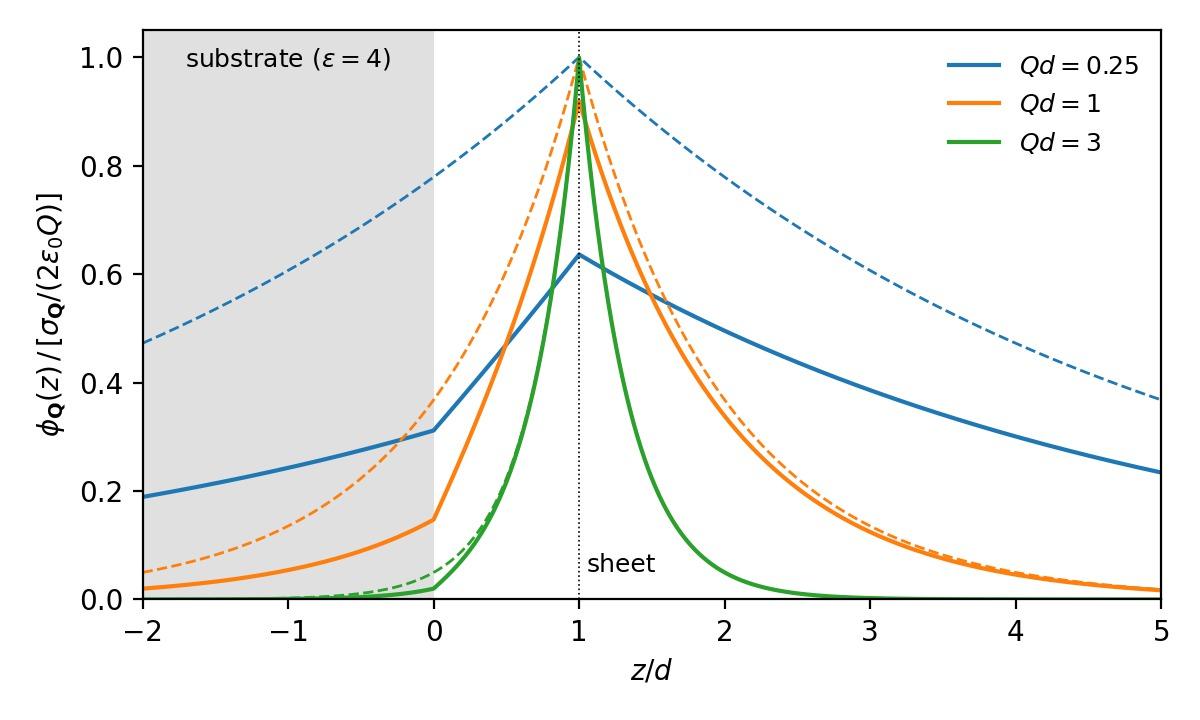
\includegraphics[width=0.75\textwidth]{Figures/sheet_potential.jpeg}
\caption{Potential of a charge wave in the plane $z = d$ above a substrate with $\varepsilon = 4$ (shaded,
$z < 0$), Eq.~\eqref{eq:phi_sub_ansatz}, for three wave vectors (solid lines). Dashed lines: free-standing sheet,
Eq.~\eqref{eq:phi_free}. The potential is in units of $\sigma_{\Qv}/(2\varepsilon_0 Q)$, its value in the plane of a
free-standing sheet. The long-wavelength wave ($Qd = 0.25$) penetrates the substrate and is strongly reduced; the
short-wavelength one ($Qd = 3$) is almost unaffected.}
\label{fig:sheet_potential}
\end{figure}

\subsection{Sheet of harmonic oscillators}
\label{sec:oscillators}

The sheet contains $n$ oscillators per unit area. Each is a particle of charge $e$ and mass $m$, bound to its site
by a harmonic force of frequency $\omega_0$, with damping $\gamma$, and free to move in the plane. In the continuum
(mean-field) description the displacement $\bm{u}$ obeys
\begin{equation}
m\left(\ddot{\bm{u}} + \gamma\dot{\bm{u}} + \omega_0^2\bm{u}\right) = e\,\bm{E}(\rpar, t) ,
\label{eq:eom}
\end{equation}
where $\bm{E}$ is the in-plane field in the sheet. For fields $\propto e^{-i\omega t}$ the dipole moment per unit
area $\bm{P} = ne\bm{u}$ is
\begin{equation}
\bm{P} = n\,\alpha(\omega)\,\bm{E} , \qquad \alpha(\omega) = \frac{e^2/m}{\omega_0^2 - \omega^2 - i\gamma\omega} ,
\label{eq:alpha}
\end{equation}
with static polarizability $\alpha(0) = e^2/(m\omega_0^2)$. A polarization wave $\bm{P}_{\Qv} e^{i\Qv\cdot\rpar}$
carries the charge $\sigma_{\Qv} = -i\Qv\cdot\bm{P}_{\Qv} = -iQP_L$, where $P_L$ is the longitudinal component
(along $\Qv$); the transverse component carries no charge and, in the quasi-static limit, produces no field. The
potential of the charge in the sheet is $\vt(Q)\sigma_{\Qv}$, Eq.~\eqref{eq:vt_sheet}, and its longitudinal field is
\begin{equation}
E^{\mathrm{ind}}_L = -iQ\,\vt(Q)\,\sigma_{\Qv} = -Q^2\,\vt(Q)\,P_L = -\frac{Q}{2\varepsilon_0\,\epsenv(Q)}\,P_L .
\label{eq:depolarization}
\end{equation}
It is a depolarization field: it opposes the polarization, it vanishes as $Q \to 0$ (charge waves of a polarization,
Sec.~\ref{sec:charge_wave}), and it is reduced by the substrate. With an external longitudinal field
$E^{\mathrm{ext}}_L$, the self-consistent polarization is
\begin{equation}
P_L = \frac{n\,\alpha(\omega)}{\varepsilon_{\mathrm{sh}}(Q,\omega)}\,E^{\mathrm{ext}}_L , \qquad
\varepsilon_{\mathrm{sh}}(Q,\omega) = 1 + \frac{Q}{2\varepsilon_0\,\epsenv(Q)}\,n\,\alpha(\omega)
= 1 - \vt(Q)\,\chi_0(Q,\omega) .
\label{eq:eps_sheet}
\end{equation}
Here $\chi_0(Q,\omega) = -Q^2 n\alpha(\omega)$ is the charge response of the oscillators to the total potential in
the plane ($\sigma_{\Qv} = \chi_0\,\phi_{\Qv}$), and $\varepsilon_{\mathrm{sh}}$ is the dielectric function of the
sheet on the substrate. Eq.~\eqref{eq:eps_sheet} has the structure of the RPA with the bare interaction replaced by
$\vt$: the response of the sheet is unchanged, and the substrate enters only through the interaction between its
charges.

\paragraph{Collective modes.} The resonances are the zeros of $\varepsilon_{\mathrm{sh}}$. For $\gamma \to 0$,
\begin{equation}
\omega_L^2(Q) = \omega_0^2 + \frac{n e^2}{2\varepsilon_0 m}\,\frac{Q}{\epsenv(Q)}
= \omega_0^2\left[1 + \frac{r_0\,Q}{\epsenv(Q)}\right] , \qquad r_0 = \frac{n\,\alpha(0)}{2\varepsilon_0} ,
\label{eq:omegaL}
\end{equation}
for the longitudinal mode, while the transverse mode stays at $\omega_T = \omega_0$. The length $r_0$ measures the
polarizability of the sheet ($r_0 = 2\pi n\alpha(0)$ in atomic units). Fig.~\ref{fig:sheet_modes}(b) shows
$\omega_L(Q)$ for $r_0 = 5d$.
\begin{itemize}
\item $Q \to 0$: $\omega_L \to \omega_0$ for any substrate. The uniform mode is not shifted, because a uniformly
  polarized sheet produces no field outside and does not polarize the substrate. Optical absorption probes
  $Q \simeq \omega/c$, many orders of magnitude below $1/d$: the resonance of the sheet on the substrate stays at
  $\omega_0$. The substrate changes the measured absorption only through the field it reflects onto the sheet
  (a retardation effect outside this model), not through a shift of the resonance.
\item Finite $Q$: the splitting $\omega_L^2 - \omega_T^2 = \omega_0^2\,r_0Q/\epsenv(Q)$ comes from the Coulomb
  coupling between the oscillators, and the substrate reduces it by the factor $1/\epsenv(Q)$, which goes from
  $2/(1 + \varepsilon)$ at $Qd \ll 1$ to 1 at $Qd \gg 1$. The longitudinal mode is softened at wavelengths larger
  than $d$.
\item Metal: $1/\epsenv \simeq 2Qd$ at small $Q$ and $\omega_L^2 \simeq \omega_0^2(1 + 2r_0dQ^2)$: the dispersion
  becomes quadratic, because the coupling between the oscillators is now short ranged.
\item Free charges, $\omega_0 \to 0$: $\omega_L^2 = ne^2Q/(2\varepsilon_0 m\,\epsenv)$, the two-dimensional plasmon,
  with the known factor $(1 + \varepsilon)/2$ of a sheet on a substrate at long wavelengths. This is a check of
  Eq.~\eqref{eq:omegaL}.
\end{itemize}

\paragraph{Static screening.} At $\omega = 0$, $\varepsilon_{\mathrm{sh}}(Q,0) = 1 + r_0Q/\epsenv(Q)$. A static
charge $\sigma^{\mathrm{ext}}_{\Qv}$ placed in the sheet produces the potential $\vt\sigma^{\mathrm{ext}}_{\Qv}$
(bare plus image), screened by the oscillators:
\begin{equation}
\phi_{\Qv} = W(Q)\,\sigma^{\mathrm{ext}}_{\Qv} , \qquad
W(Q) = \frac{\vt(Q)}{\varepsilon_{\mathrm{sh}}(Q,0)} = \frac{1}{2\varepsilon_0 Q\left[\epsenv(Q) + r_0Q\right]} .
\label{eq:W_keldysh}
\end{equation}
This is the Keldysh form of the screened interaction in a thin layer, with the environment described by
$\epsenv(Q)$ and the screening length $r_0$ given by the polarizability of the oscillators. It is the interaction
felt by a charge added to the sheet, which is the subject of the GW problem.

\begin{figure}[h!]
\centering
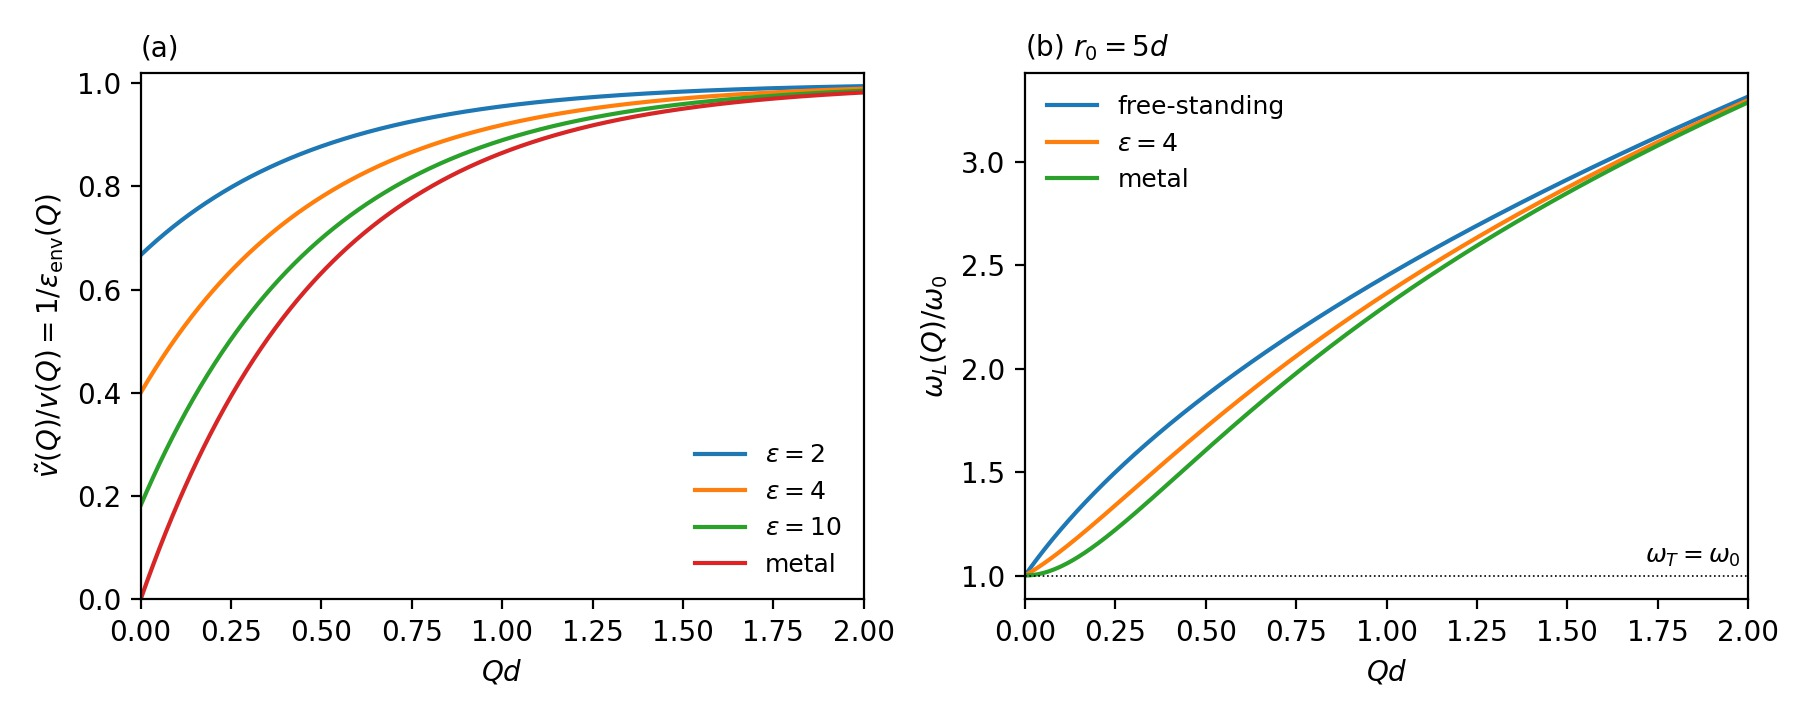
\includegraphics[width=\textwidth]{Figures/sheet_modes.jpeg}
\caption{(a) Ratio between the dressed and the bare Coulomb interaction in the plane of the sheet,
Eq.~\eqref{eq:vt_sheet}, for several substrates. (b) Longitudinal mode of the sheet of oscillators,
Eq.~\eqref{eq:omegaL}, for $r_0 = 5d$: free-standing ($\varepsilon = 1$), on a dielectric with $\varepsilon = 4$
and on a metal. The transverse mode is at $\omega_0$ in all cases.}
\label{fig:sheet_modes}
\end{figure}

\subsection{Discreteness and the single oscillator}
\label{sec:single}

The continuum description replaces the field acting on each oscillator by the field of a smoothly polarized sheet.
The opposite limit is a single oscillator at height $d$, far from the others. A point charge $e$ above the
substrate has an image $-\beta e$ at the mirror position; hence an in-plane dipole $\bm{p}$ has the image dipole
$-\beta\bm{p}$, and a dipole $p_z$ normal to the surface has the image $+\beta p_z$. The field of the image at the
oscillator (distance $2d$ along $z$) is parallel to the dipole, $\beta p/(32\pi\varepsilon_0 d^3)$ for the in-plane
dipole and $\beta p_z/(16\pi\varepsilon_0 d^3)$ for the normal one. It adds to the restoring force in
Eq.~\eqref{eq:eom} with the opposite sign, so the resonance is red shifted:
\begin{equation}
\omega_{\parallel}^2 = \omega_0^2\left[1 - \frac{\beta\,\alpha(0)}{32\pi\varepsilon_0 d^3}\right] , \qquad
\omega_{\perp}^2 = \omega_0^2\left[1 - \frac{\beta\,\alpha(0)}{16\pi\varepsilon_0 d^3}\right] .
\label{eq:single_shift}
\end{equation}
This is the interaction of a fluctuating dipole with its own image, the classical counterpart of the van der Waals
shift of an atomic transition near a surface. It decays as $1/d^3$ and is small: for a polarizability volume
$\alpha(0)/4\pi\varepsilon_0$ of a few \AA$^3$, $d = 3$~\AA\ and $\beta \simeq 0.6$,
$\Delta\omega_{\parallel}/\omega_0 \simeq -\beta\alpha(0)/(64\pi\varepsilon_0 d^3)$ is below one percent.

For a dense sheet the images of all the oscillators act together. For oscillators on a lattice with sites
$\bm{R}$ and a mode $\bm{P}\,e^{i\Qv\cdot\bm{R}}$, the sum over the lattice of the image fields can be written, by
Poisson summation, as a sum over the reciprocal lattice vectors $\bm{G}$: the term $\bm{G} = 0$ is the continuum
result above, and the terms $\bm{G} \neq 0$ are reduced by $e^{-2|\Qv + \bm{G}|d}$. For a hexagonal lattice with
$a = 4$~\AA\ ($|\bm{G}_{\min}| = 4\pi/\sqrt{3}a \simeq 1.8$~\AA$^{-1}$) and $d = 3$~\AA, this factor is about
$2\times10^{-5}$: the image of each oscillator is compensated by the images of its neighbours, and the continuum
description is accurate. The same decomposition of the direct field of the other oscillators in the plane gives,
besides the continuum term, a local-field correction that does not depend on the substrate; we take it as included
in $\omega_0$. The single-oscillator shift of Eq.~\eqref{eq:single_shift} is recovered only when the oscillators
are farther apart than $d$.

\subsection{What the model shows}
\label{sec:modelA_summary}

\begin{itemize}
\item The substrate does not change the oscillators: it changes the Coulomb interaction between them, $v \to \vt$,
  and only for wavelengths larger than about $d$.
\item The uniform (optical) mode of the sheet is not shifted; the longitudinal modes at finite $Q$ are softened,
  because the substrate screens the Coulomb coupling between the oscillators.
\item A neutral and localized excitation feels the substrate only through the image of its dipole, a relative
  effect of order $\alpha(0)/(4\pi\varepsilon_0 d^3)$ that is cancelled by the neighbours in a dense sheet.
\item A net charge in the sheet interacts instead with its own image, an effect of order $e^2/(4\pi\varepsilon_0 d)$
  (the constant $-\beta/(8\pi\varepsilon_0 d)$ of Eq.~\eqref{eq:vt_real} at short distance), screened by the
  oscillators through Eq.~\eqref{eq:W_keldysh}. Charged excitations, and pairs of opposite charges at a finite
  distance, are not described by this model: they are needed to see the renormalization of the quasiparticle gap
  and of the exciton binding energy.
\end{itemize}

\bibliographystyle{unsrt}
\bibliography{biblio}

\end{document}
